% ---------------------------------------------------------------------------
% Architecture figure for architecture.tex (Section: System Architecture).
%
% Requires \usepackage{graphicx}. The figure is 7 in wide, so it spans both
% columns: use figure* as below. If you would rather keep it inside one column,
% regenerate at figsize=(3.4, 4.6) in figures/make_architecture_fig.py and
% change figure* to figure.
%
% Prefer the PDF for camera-ready (vector, no resampling); the PNG is bundled
% at 400 dpi for drafts and for reviewers who compile with a PNG-only path.
%
% Suggested placement: in \subsection{Overview}, insert the FIGURE below the
% \begin{table}[t] block, and the PARAGRAPH immediately after the paragraph
% ending "...the monitor and the records manager aggregate." (line 22).
% ---------------------------------------------------------------------------

\begin{figure*}[t]
\centering
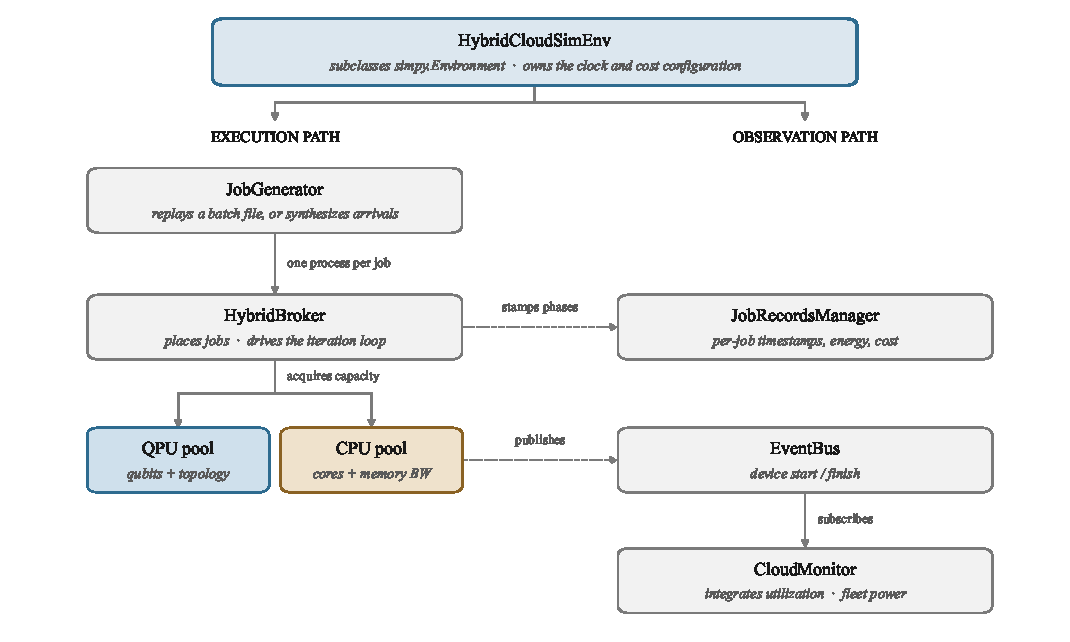
\includegraphics[width=\textwidth]{figures/architecture}
\caption{Component structure of HybridCloudSim. Both paths descend from the
composition root, but they never join: the execution path (left) places jobs
and consumes device capacity, while the observation path (right) only records
what the execution path has already committed. Dashed links carry telemetry
and never influence placement.}
\label{fig:architecture}
\end{figure*}


% --- paragraph to accompany the figure -------------------------------------

Figure~\ref{fig:architecture} makes this separation explicit. The execution and
observation paths descend from the same root but never join: the broker
consults device capacity in order to place work, whereas the event bus, the
cloud monitor, and the records manager only ever read state that the execution
path has already committed. No scheduling decision depends on a telemetry
value. This asymmetry is what allows instrumentation to be as dense as the
analysis requires --- every phase transition of every job is stamped, and every
device transition is published --- without perturbing the schedule under study.
It also fixes the provenance of each reported quantity: phase boundaries
originate in the broker, device arrivals in the devices themselves,
time-integrated utilization and instantaneous fleet power in the monitor, and
per-job energy and cost in the records manager. We rely on that provenance in
Section~\ref{sec:arch-telemetry}, where the two independently computed energy
figures are reconciled.
